\documentclass[russian,ukrainian,utf8,floatsection,equationsingle,14pt,simple]{eskdtext}

\usepackage{eskddstu}

% \usepackage{eskdchngsheet}
\usepackage[T2A]{fontenc}
\usepackage[utf8]{inputenc}
% \geometry{left=3cm}
%\usepackage{cyrtimes}
\usepackage{pscyr}
\usepackage{mathtext}
\usepackage{tabularx}
\usepackage{multirow}
\usepackage{listings}
\usepackage{setspace}
\usepackage{amsmath}
\usepackage{amssymb}
\usepackage{graphicx}
\usepackage{verbatim}
\usepackage{indentfirst}
\usepackage{lscape}
\usepackage{paralist}
\usepackage{gost}
\usepackage{longtable}
\usepackage[thmmarks,amsmath]{ntheorem}
\usepackage[unicode]{hyperref}
\usepackage{algorithm2e}

\usepackage{svg}

\usepackage{rotating}
\usepackage{ulem}
\usepackage{cancel}
%Чтобы ссылки автоматически не вставлялись под \path
\def\BibUrl#1{#1} 
% \ESKDsectStyle{section}{\Large\bfseries}
% \ESKDsectAlign{section}{Center}
\ESKDsectSkip{section}{5pt}{10pt}
\ESKDsectSkip{subsection}{5pt}{5pt}
\ESKDsectSkip{subsubsection}{0pt}{5pt}
\renewcommand{\baselinestretch}{1.5} % Задаём единичный межстрочный интервал

% vim: nocindent:

\hyphenation
{
  Open-FOAM
  ал-го-рит-мів
  ал-го-рит-мом
  ал-го-рит-му
  апро-кси-ма-ція-ми
  біб-ліо-те-ка
  век-тор
  век-то-ри
  век-то-рів
  виг-ля-ді
  від-нос-но
  від-по-ві-да-ють
  влас-ний
  влас-них
  вуз-ла
  вхід-них
  дея-кі
  до-дат-ко-ві
  ефек-тив-ним
  зас-то-со-вує-ться
  зруч-но-му
  ка-фед-рою
  квад-рат
  квад-рат-ної
  ква-лі-фі-ка-цій-но
  клас-тер-ної
  кое-фі-ці-єнт
  мак-си-маль-ної
  мат-ри-ці
  мат-риць
  мат-ри-ця
  мож-ли-вим
  нас-туп-ні
  не-мож-ли-во
  об-роб-ля-ти
  об-чис-ленні
  об-чис-лення
  об-чис-лень
  об-чис-лю-валь-ни-ми
  об-чис-лю-валь-но
  об-чис-лю-валь-ної
  пе-ре-тво-рен-ня
  пос-лі-дов-нос-ті
  прак-тич-не
  пре-фікс-ної
  про-дук-тив-ність
  різ-но-ма-ніт-них
  роз-рід-же-ної
  си-ме-трич-них
  си-ме-трич-ної
  сис-тем
  сис-те-мі
  склад-ність
  склад-но-сті
  цик-лу
}

\ESKDdepartment{Міністерство освіти і науки України}
\ESKDcompany{Національний технічний університет України%
<<Київський політехнічний інститут>>}

\ESKDauthor{Уварова~Н.\,В.}
%\ESKDchecker{Стіренко~С.\,Г.}
%\ESKDnormContr{Симоненко~В.\,П.}
%\ESKDapprovedBy{Луцький~Г.\,М.}
\ESKDdate{2012/01/16}
\ESKDcolumnIX{НТУУ <<КПІ>> ФІОТ ІО-82}

% Set text padding
\ESKDsetPadding{10mm}{10mm}

% Redefine TOC styles
\makeatletter
\renewcommand{\l@section}{\@dottedtocline{0}{1.5em}{2.3em}}
\renewcommand{\l@subsection}{\@dottedtocline{1}{2.5em}{2.3em}}
\renewcommand{\l@subsubsection}{\@dottedtocline{2}{3.5em}{2.3em}}
\makeatother

% Document separator
\newcommand{\docseparator}[1]{
  \newpage
  \thispagestyle{empty}
  \ESKDthisStyle{empty}
  \noindent\parbox[c][\vsize][c]{\hsize}
  {\centering\fontsize{36pt}{40pt}\selectfont#1}

  % reset all counters
  \setcounter{page}{0}
  \setcounter{section}{0}
  \setcounter{subsection}{0}
  \setcounter{subsubsection}{0}
}

\newcommand{\apptitletop}[1]{%
ДОДАТОК #1\par
Алгоритм динамічної маршрутизації мультікастової розсилки}

\newcommand{\apptitlepages}[1]{%
Аркушів \pageref{LastPage}\par}

% Appendix title page
\newcommand{\appendixtitle}[3]{
  \newpage
  \thispagestyle{empty}
  \ESKDthisStyle{empty}
  \noindent
  \parbox[t][0.15\vsize][t]{\hsize}
  {\centering\large\apptitletop{#1}}
  \parbox[t][0.4\vsize][c]{\hsize}
  {\centering\Large\textbf{#2}\par#3}
  \parbox[t][0.20\vsize][c]{\hsize}{~~}
  \parbox[t][0.08\vsize][t]{\hsize}
  {\centering\apptitlepages}
  \vfill
  \noindent\parbox[c]{\hsize}{\centering\titlebottom}

  % reset all counters
  \setcounter{page}{0}
  \setcounter{section}{0}
  \setcounter{subsection}{0}
  \setcounter{subsubsection}{0}
}

% Header
\newcommand{\titletop}{%
\textbf{МІНІСТЕРСТВО ОСВІТИ І НАУКИ УКРАЇНИ}\par
\textbf{НАЦІОНАЛЬНИЙ ТЕХНІЧНИЙ УНІВЕРСИТЕТ УКРАЇНИ}\par
\textbf{<<КИЇВСЬКИЙ ПОЛІТЕХНІЧНИЙ ІНСТИТУТ>>}\par
Факультет інформатики і обчислювальної техніки\par
Кафедра обчислювальної техніки}

\newcommand{\titledocname}{%
БАКАЛАВРСЬКА ДИПЛОМНА РОБОТА\par
НА ТЕМУ}

\newcommand{\titledocnameI}{%
БАКАЛАВРСЬКА ДИПЛОМНА РОБОТА}

\newcommand{\titledocnameII}{%
БАКАЛАВРСЬКА ДИПЛОМНА РОБОТА\par
НА ТЕМУ}

\newcommand{\titleregistry}{%
\textbf{Реєстраційний \No} \underline{~~~~~~~~~~}}

\newcommand{\titlescript}{%
\textbf{На правах рукопису}\par
УДК \underline{~~~~~~~~~~~~~~~~~~~~}}

\newcommand{\titleapproveI}{%
\textbf{Затверджую}\par
зав. кафедрою, д.т.н., проф.\par
\underline{~~~~~~~~~~~~~~~} (Луцький~Г.\,М.)\par
\vspace{-3mm}{\small(підпис, дата)}}

\newcommand{\titleapproveII}{%
\textbf{Узгоджено}\par
Науковий керівник\par
к.т.н., доц.\par
Стіренко Сергій Григорович\par
~\par
\underline{~~~~~~~~~~~~~~~~~~~~~~~~~~~~~}\par
\vspace{-3mm}{\small~~~~~~~~(підпис, дата)}}

\newcommand{\titledefence}{%
Захищено <<\underline{~~~}>> \underline{~~~~~~~~~~} 2012 р.\par
З оцінкою \underline{~~~~~~~~~~~~~~~}\par
Члени комісії\par
\underline{~~~~~~~~~~~~~~~~~~~~~~~~~~~~~}\par
\vspace{2mm}\underline{~~~~~~~~~~~~~~~~~~~~~~~~~~~~~}\par
\vspace{2mm}\underline{~~~~~~~~~~~~~~~~~~~~~~~~~~~~~}}

\newcommand{\titletheme}{%
\textbf{\underline{Реалізація задачі знаходження власних чисел та векторів}}\par
\textbf{\underline{методом Ланцоша на кластерній системі}}}

\newcommand{\titlesubtheme}{%
Зі спеціальності (за напрямком) 6.050102\par
<<Комп'ютерна інженерія>>}

\newcommand{\titleauthorI}{%
\textbf{Виконавець роботи}\par
ФІОТ, гр. ІО-72\par
номер залікової книжки: 7202\par
Грибенко Дмитро В'ячеславович\par
\vspace{2mm}\underline{~~~~~~~~~~~~~~~~~~~~~~~~~~~~~}\par
\vspace{-3mm}{\small~~~~~~~~(підпис, дата)}}

\newcommand{\titleauthorII}{%
\textbf{Виконавець роботи}\par
Грибенко Дмитро В'ячеславович\par
\vspace{2mm}\underline{~~~~~~~~~~~~~~~~~~~~~~~~~~~~~}\par
\vspace{-3mm}{\small~~~~~~~~(підпис, дата)}}

\newcommand{\titleadviser}{%
\textbf{Науковий керівник}\par
к.т.н., доц.\par
Стіренко Сергій Григорович\par
~\par
\vspace{2mm}\underline{~~~~~~~~~~~~~~~~~~~~~~~~~~~~~}\par
\vspace{-3mm}{\small~~~~~~~~(підпис, дата)}}

\newcommand{\titlebottom}{%
Київ 2012~р.}

\renewcommand{\maketitle}{
  \thispagestyle{empty}
  \ESKDthisStyle{title}

  \noindent\parbox[c][0.15\vsize][t]{\hsize}
  {\begin{center}\titletop\end{center}}
  \parbox[t][0.08\vsize][t]{\hsize}
  {
    \parbox[t]{0.4\hsize}{\raggedright\titleregistry}\hfill
    \parbox[t]{0.4\hsize}{\raggedright\titlescript}
  }
  \parbox[t][0.1\vsize][t]{\hsize}
  {
    \parbox[t]{0.4\hsize}{\raggedright}\hfill
    \parbox[t]{0.4\hsize}{\raggedright\titleapproveI}
  }
  \parbox[t][0.05\vsize][c]{\hsize}{~~}
  \parbox[t][0.08\vsize][c]{\hsize}
  {\begin{center}\titledocname\end{center}}
  \parbox[t][0.08\vsize][c]{\hsize}
  {\begin{center}\titletheme\end{center}}
  \parbox[t][0.08\vsize][c]{\hsize}
  {\begin{center}\titlesubtheme\end{center}}
  \parbox[t][0.08\vsize][c]{\hsize}{~~}
  \parbox[t][0.2\vsize][t]{\hsize}
  {
    \parbox[t]{0.45\hsize}{\raggedright\titleauthorI}\hfill
    \parbox[t]{0.4\hsize}{\raggedright\titleadviser}
  }
  \vfill
  \begin{center}\titlebottom\end{center}
}

\newcommand{\maketitleI}{
  \thispagestyle{empty}
  \ESKDthisStyle{title}

  \noindent\parbox[c][0.20\vsize][t]{\hsize}
  {\centering\titletop}
  \parbox[t][0.07\vsize][t]{\hsize}
  {
    \parbox[t]{0.4\hsize}{\raggedright\titleregistry}\hfill
    \parbox[t]{0.4\hsize}{\raggedright\titlescript}
  }
  \parbox[t][0.15\vsize][t]{\hsize}
  {
    \parbox[t]{0.4\hsize}{\raggedright}\hfill
    \parbox[t]{0.4\hsize}{\raggedright\titleapproveI}
  }
  \parbox[t][0.08\vsize][c]{\hsize}
  {\centering\titledocnameI}
  \parbox[t][0.08\vsize][c]{\hsize}
  {\centering\titlesubtheme}
  \parbox[t][0.12\vsize][c]{\hsize}{~~}
  \parbox[t][0.2\vsize][t]{\hsize}
  {
    \parbox[t]{0.45\hsize}{\raggedright\titleauthorI}\hfill
    \parbox[t]{0.4\hsize}{\raggedright\titleadviser}
  }
  \vfill
  \noindent\parbox[c]{\hsize}{\centering\titlebottom}
}

\newcommand{\maketitleII}{
  \thispagestyle{empty}
  \ESKDthisStyle{title}

  \noindent\parbox[c][0.15\vsize][t]{\hsize}
  {\centering\titletop}
  \parbox[t][0.20\vsize][t]{\hsize}
  {
    \parbox[t]{0.45\hsize}{\raggedright\titleapproveII}\hfill
    \parbox[t]{0.45\hsize}{\raggedright\titledefence}
  }
  \parbox[t][0.05\vsize][c]{\hsize}{~~}
  \parbox[t][0.08\vsize][c]{\hsize}
  {\centering\titledocnameII}
  \parbox[t][0.08\vsize][c]{\hsize}
  {\centering\titletheme}
  \parbox[t][0.08\vsize][c]{\hsize}
  {\centering\titlesubtheme}
  \parbox[t][0.10\vsize][c]{\hsize}{~~}
  \parbox[t][0.2\vsize][t]{\hsize}
  {
    \parbox[t]{0.45\hsize}{\raggedright}\hfill
    \parbox[t]{0.45\hsize}{\raggedright\titleauthorII}
  }
  \vfill
  \noindent\parbox[c]{\hsize}{\centering\titlebottom}
}

\makeatletter
\newcommand\bigpart[1]{%
  \begingroup%
  \ESKDsectAlign{section}{Center}%
  \section*{#1%
    \@mkboth{%
      \MakeUppercase#1}{\MakeUppercase#1}}%
  \addcontentsline{toc}{section}{#1}%
  \endgroup}
\newcommand\bignotocpart[1]{%
  \begingroup%
  \ESKDsectAlign{section}{Center}%
  \section*{#1%
    \@mkboth{%
      \MakeUppercase#1}{\MakeUppercase#1}}%
  \endgroup}
\newcommand\bignumberedpart[1]{%
  \begingroup%
  \ESKDsectAlign{section}{Center}%
  \stepcounter{section}%
  \section*{Розділ \arabic{section}}%
  \vspace{-5mm}%
  \section*{#1%
    \@mkboth{%
      \MakeUppercase#1}{\MakeUppercase#1}}%
  \addcontentsline{toc}{section}{Розділ \arabic{section}. #1}%
  \endgroup}
\makeatother

\newcommand{\vect}[1]{\mathbf{#1}}
\DeclareMathOperator{\const}{const}
\DeclareMathOperator{\proj}{\mathbf{proj}}
\DeclareMathOperator{\rang}{\mathbf{rang}}
\DeclareMathOperator{\opspan}{\mathbf{span}}
\DeclareMathOperator{\opdim}{\mathbf{dim}}
\DeclareMathOperator*{\argmin}{arg\,min}

% theorem-like environments
\theoremstyle{plain}
\theorembodyfont{}
\theoremseparator{.}
\newtheorem{example}{Приклад}
\newtheorem{theorem}{Теорема}

\theoremstyle{nonumberplain}
\theoremseparator{.}
\theoremsymbol{\rule{1ex}{1ex}}
\newtheorem{proof}{Доведення}

\numberwithin{equation}{section}
\numberwithin{theorem}{section}
\numberwithin{figure}{section}
\numberwithin{table}{section}

\makeatletter
% \def\verbatim@font{\fontfamily{fcr}\fontsize{10pt}{11pt}\selectfont\@noligs}
\makeatother

% remove some hyperref warnings
\makeatletter
\providecommand*{\toclevel@theorem}{0}
\providecommand*{\toclevel@proof}{0}
\makeatother

\newcommand\algorule{\rule{\textwidth}{0.5pt}}

% inline program code
\newcommand{\icode}[1]{\texttt{\small#1}}

% zero-width space (allow breaking lines)
\newcommand{\zwsp}{\hspace{0mm}}


% to be done block
\usepackage{color}
\newcommand{\TBD}{{\color{red}To be done}}

\ESKDsignature{IАЛЦ.467200.003 ПЗ}
% \newcommand{\docseparator}[1]{
%   \newpage
%   \thispagestyle{empty}
%   \ESKDthisStyle{empty}
%   \noindent\parbox[c][\vsize][c]{\hsize}
%   {\centering\fontsize{36pt}{40pt}\selectfont#1}
% 
%   % reset all counters
%   \setcounter{page}{0}
%   \setcounter{section}{0}
%   \setcounter{subsection}{0}
%   \setcounter{subsubsection}{0}
% }

\renewcommand{\labelenumi}{\arabic{enumi}. }

\begin{document}

% \maketitleII

% Fit the abstract on a single page
% \ESKDsetPadding{7mm}{4mm}

\newcommand{\abstracttile}[1]{%
\begingroup%
\centering\fontsize{18pt}{20pt}\selectfont\textbf{#1}\par%
\endgroup}

\thispagestyle{empty}
\ESKDthisStyle{empty}
% \linespread{1.05}\selectfont
\abstracttile{Анотація}
У даній бакалаврській роботі розглянуті питання виявлення аномалій в поведінці абонентів телефонної мережі. Досліджені різні способи виявлення аномалій. Розроблений спосіб виявлення аномалій на базі моделі Денінга, запропоновано модифікацію способу для врахування групових змін в поведінці абонентів.

Розроблена програма для виявлення аномалій абонентів телефонної мережі, досліджено роботу алгоритму у режимах без модифікації та з модифікацією.

\abstracttile{Аннотация}
В данной бакалаврской работе рассмотрены вопросы обнаружения аномалий в поведении абонентов телефонной сети. Исследованы различные способы выявления аномалий. Разработан способ обнаружения аномалий на базе модели Деннинга, предложена модификация способа для учета групповых изменений в поведении абонентов.

Разработана программа для обнаружения аномалий в поведении абонентов телефонной сети, исследована работа алгоритма в режимах без модификации и с модификацией.

\abstracttile{Abstract}
In this work the problem of detection anomalies in the behavior of telephone subscribers is studied. Various methods of anomaly detection are analyzed. The method of anomaly detection is developed, approach of improving method to take into consideration group behavior changes is proposed.

The program for detecting anomalies in subscriber behavior is developed, results of simulation in two modes, with and without modification, are given.


\lstset{
numbers=none,
basicstyle=\footnotesize,
numberstyle=\tiny,
tabsize=4,
breaklines=true,
title=\lstname
}
\docseparator{Пояснювальна\\записка}

\newpage

\ESKDthisStyle{formII}
\tableofcontents
\newpage
% \section*{Список скорочень}
\newpage
\bigpart{Перелік умовних позначень}
% \addcontentsline{toc}{section}{Список скорочень}
%    OSPF - Open Shortest Path First
\begin{ESKDexplanation}
  \item АТС --- Автоматична телефонна станція
  \item ADS --- Anomaly Detection System
  \item CDR --- Call Detail Record
  \item HDFS --- Hadoop File System
  \item IDS --- Intrusion Detection System
  \item MDS --- Misuse Detection System
  \item PBX --- Private Branch eXchange
  \item SIP --- Session Initiation Protocol
\end{ESKDexplanation}

% \section*{Вступ}
%notoc \addcontentsline{toc}{section}{Вступ}
\newpage
\bigpart{Вступ}

\TBD \cite{rader2014cdr}.
\TBD \cite{rader2014cdr}.

% \newpage
\bignumberedpart{Постановка задачі виявлення аномалій у поведінці користувачів}

\subsection{Опис предметної області}
  Останнім часом в світі переконались, що навіть найнадійніші системи захисту не здатні захистити від атак комп'ютерні системи державних і комерційних установ. Одна з причин - у тому, що в більшості систем безпеки застосовують стандартні механізми захисту: ідентифікацію та аутентифікацію, механізми обмеження доступу до інформації згідно з правами суб'єкта і криптографічні механізми. Такий традиційний підхід має певні недоліки, а саме: незахищеність від власних користувачів - зловмисників, розмитість поділу суб'єктів системи на "своїх" і "чужих" через глобалізацію інформаційних ресурсів, порівняна легкість підбору паролів внаслідок використання їхнього змістового різновиду, зниження продуктивності й ускладнення інформаційних комунікацій внаслідок обмеження доступу до ресурсів організації. Тому виникла потреба в механізмах, які би доповнювали традиційні та давали можливість виявити спроби несанкціонованого доступу й інформували про це відповідальних за безпеку або реагували у відповідь. Важливим фактором є те, щоб такі системи могли протистояти атакам, навіть якщо зловмисник вже був аутентифікований та авторизований і з формального погляду додержання прав доступу мав необхідні повноваження на свої дії. Такі функції і виконують системи виявлення вторгнень IDS (intrusion detection systems). Оскільки передбачити всі сценарії розгортання подій в системі з активним "чужим"  
  суб'єктом неможливо, потрібно або якомога детальніше описати можливі "зловмисні" сценарії або ж, навпаки, - "нормальні" і прийняти, що всяка активність, на яку не поширюється прийняте розуміння "нормальності", є небезпечною. Системи IDS поділяються на системи, що реагують на відомі атаки, - системи виявлення зловживань MDS (misuse detection systems) і системи виявлення аномалій ADS (anomaly detection systems), які реєструють відхилення розвитку системи від нормального перебігу. \TBD

\subsection{Приклади вторгнення}

	Розглянемо офісну міні-АТС (PBX), яка обслуговує телефонних абонентів одного або кількох офісних приміщень або будинків. В результаті використання ресурсів неавторизованим користувачем, або авторизованим нелегально, можуть бути вагомі неотримані прибутки компанією оператором. Ці неотримані прибутки можуть бути покладені на абонентом (в даному випадку абонентом є компанія-замовник АТС, де кінцевими абонентами є співробітники компанії), АТС якого був використаний нелегально. В разі доведення абонентом (можливо в судовому порядку), що втрати були понесені внаслідок атаки, оператор може не отримати ці кошти, хоча послуга вже отримана та зроблені витрати на надання послуги.

	Розглянемо телефонну мережу оператора стаціонарного чи мобильного зв'язку. В такій мережі існує велика кількість АТС (PBX), розподілених по території та які обслуговують велику кількість абонентів. Внаслідок нелегального використання послуг оператор може понести великі операційні збитки, а також істотні збитки у судових справах.

\subsection{Основні поняття}

  Система виявлення вторгнень - програмний або апаратний засіб, призначений для виявлення фактів несанкціонованого доступу в мережу або несанкціонованого управління ними в основному через Інтернет. Відповідний англійський термін - Intrusion Detection System (IDS).

  Для запобігання шахрайству у мережах використовують мережеві екрани, що можуть блокувати або дозволяти певний трафік через себе.
  Основна різниця між мережевим екраном (файрволом) та системою виявлення вторгнення полягає у області дії. Мережевий екран діє на границі мережі, тоді як система виявлення вторгнень - всередені, вона пропускає через себе весь трафік та виявляє аномальні ділянки.

	Наразі існують два доступних види телефонних комунікацій. Перший це наземні аналогові лінії, які передають неперервний хвилевий сигнал, другий використовує цифрову передачу сигналу, в якому трафік кодується за допомогою швидкої передачі бінарних імпульсів. На даний момент оператори мобільного зв'язку використовують цифровий спосіб передаці голосових даних та більшість операторів наземного перейшли на цифрові системи.

	Протокол SIP у телефонії використовується майже скрізь, цифрові системи АТС (PBX) характеризуються легкістю аналізу даних. Call Detail Record (CDR), також відомий як запис даних виклику, є записом у журналі телефонної станції або іншого телекомунікаційного обладнання, що містить атрибути, характерні для одного телефонного дзвінка або іншої послуги зв'язку, яка була оброблена системою.

	Види шахрайства та втручання в систему були досліджені у роботі \cite{barson1996detection} та компанією TransNexus \cite{transnexus2012voipfraud},

\begin{itemize}
  \item Клонування телефонів - отримання доступу до мережі шляхом емуляції ідентифікаційного коду
другого справжнього мобільного телефону. Дані, що містяться на чіпі мобільного телефону (або SIM-картці) копіюються з одного мобільного телефону на інший. Цей тип шахрайства можна виявити в пересіченні телефонних дзвінків у часі,
  \item Шахрайство при підключенні - використання фальшивих ідентифікаційних даних для підключення до мережі. Цей тип шахрайства зазвичай не може бути визначений до першого зняття грошей з рахунку. Дані підключення також можуть бути скопійовані, тоді у мережі будуть присутні кілька телефонів, підключених з одними ідентифікаційними даними,
  \item Крадіжка телефону - легитимний власник телефону втрачає можливість робити дзвінки, а витрати робить неавторизована особа,
  \item Злам АТС - зазвичай використовується для виконання міжнародних дзвінків через чужу телефонну станцію. шахраї можуть використовувати вразливості у ПЗ АТС та можуть згенераувати значну кількість трафіку,
  \item Дзвінки на нерозподілені номери - шахраї можуть штучно створювати неіснуючі напрямки дзвінків та реєструватися єдиними провайдерами, що можуть з'єднати з номерами цих напрямків. Створюючи трафік на такі неіснуючі номери, дзвінки будуть перенаправлятися на компанію-шахрая.
\end{itemize}

Основними моментами для визначення втручання у систему можна визначити \cite{barson1996detection}:

\begin{itemize}
  \item Шахрайство є динамічним за своєю природою: нечесна поведінка буде змінюватися з плином часу,
  \item Розмірність задачі є достатньо великою за рахунок кількості абонентів, що мають бути відслідковані одночасно,
  \item Швидке виявлення шахрайства необхідно: збитки від шахрайства, як правило, ростуть експоненційно \cite{bliss1993fraud},
  \item Система має бути прозорою, клієнт не повинен бачити систему виявлення шахрайства в дії. Система виявлення аномалій не повинна бути максимально розумною, щоб надавати найменшу кількість хибно-позитивних та хибно-негативних сигналыв, але і не має бути автоматичною. Телефон не має бути заблокований, якщо немає достатньої впевненості, що це є зловмисник.
\end{itemize}

\subsection{Формальна постановка задачі}


	Розглянемо потік подій $\{T_i\}, i = \overline{1..n}$, де кожна подія $T_i$ характеризується кортежем
  \begin{equation}\label{eq:tuple} (src, time) \end{equation}
  \begin{ESKDexplanation}
    \item де src -- номер абонента, що ініціював дзвінок;
    \item time -- час ініціювання дзвінка.
  \end{ESKDexplanation}

  Кожен абонент має унікальний номер $src$, за яким його можна ідентифікувати. Задача розроблюваного алгоритму та системи - визначити у реальному часі чи є потік подій для конкретного абонента аномальним, чи співпадає із очікованим шаблоном поведінки.

  \begin{equation}\label{eq:stream}\{T_i^{p}\} = \{x | x \in T_i \wedge x_1 = p\}\end{equation}
  \begin{ESKDexplanation}
    \item де p - номер телефону.
  \end{ESKDexplanation}

  Тоді потік можна записати як сукупність потоків 

  \begin{equation}\label{eq:stream_sum}\{T_i\} = \{T_i^{p_1}\} \cup \{T_i^{p_2}\} \cup ... \cup \{T_i^{p_k}\} \end{equation}
  \begin{ESKDexplanation}
    \item де k - кількість телефонних номерів.
  \end{ESKDexplanation}

  Шаблон поведінки користувача - функція, що показує інтенсивність дзвінків від часу
  \begin{equation}\label{eq:pattern}P: t \rightarrow \lambda \end{equation}

  \begin{ESKDexplanation}
    \item де $\lambda$ - це кількість дзвінків на одиницю часу.
  \end{ESKDexplanation}

  Для кожного моменту часу $t$ можна визначити частоту, де шаблонна частота 
\begin{equation}\label{eq:pattern_freq} \lambda_t^p = P^p(t) \end{equation}

  а фактична частота
 \begin{equation}\label{eq:real_freq} \lambda_{rt}^p = F(\{T_i^p\}) \end{equation}
 \begin{ESKDexplanation}
    \item де $F$ - це функція розрахунку поточної частоти дзвінків.
  \end{ESKDexplanation}

  Задача 1: Сформувати шаблони поведінки для кожного номеру за історією подій: $\{T_i^{p}\} \rightarrow P^{p}$.

  Задача 2: Визначити функцію $F({T_i^p})$ (\ref{eq:real_freq}) На базі cформованих шаблонів поведінки $P^{p}$ та потоку подій $\{T_i\}, i = \overline{1..n}$ визначити чи є подія $T_{n+1}$ аномальною.

\newpage
\subsection*{Висновки до розділу 1}
\addcontentsline{toc}{subsection}{Висновки до розділу 1}
    \TBD



\newpage
\bignumberedpart{Огляд існуючих розв'язків}
\subsection{Модель системи виявлення вторгнень в реальному часі}
\subsubsection{Принцип роботи}
Система виявлення вторгнення в реальному часі базується на гіпотезі, що експлуатація вразливостей системи включає аномальне використання системи. Тому, порушення безпеки можуть бути виявлені як аномальні використання системи \cite{denning1987intrusion}.

Модель системи заснована на правилах перевірки відповідності шаблону. Коли створюється запис аудиту, він порівнюється з профілями користувачів, додає інформацію у відповідні профілі, потім визначає, які правила застосовувати для оновлення профілів, перевірки аномальної поведінки і як повідомляти, що аномалії виявлені. Щаблони профілів визначаються оператором з системи моніторингу, але правила і профілі структури в певній мірі незалежні від системи. % у меня не так, у меня профили тоже делает система (только отдельный модуль)

Основна ідея полягає в спостереженні за стандартними операціями у цільовій системі: входи, команди, запуск програм, доступ до файлів і пристроїв і т.д. Модель не містить будь-яких особливих механізмів для визначення складних дій, які використовують відомі або підозрілі дефекти в безпеці цільової системи; дійсно, система не має ніяких знань про механізми безпеки на цільовій системі або їх недоліки. Хоча механізм виявлення вторгнень на основі відомих або підозрілих дефектів може бути достатьно ефективним, було б значно складніше упоратися із вторгненнями, які використовують недоліки, що не підозрюються або с пов'язані із персоналом, який обслуговує цільову систему.

\subsubsection{Реалізація / мат.модель ?\TBD}

Профілі активності характеризують поведінку суб'єктів, тобто слугує "підпісом", або описом нормальної поведінки суб'єктів. Зауважена поведінка характеризується в рамках статистичних метрик та моделей. Метрика - випадкова змінна $x$, що характеризує дискретну величину - кількість відповідних подій, що пройшли за певний період часу. Період може бути фіксований, або між двома іншими подіями (вхід та вихід з системи). Спостереження (вибірка) дістається із записів аудиту системи (журналу) та за допомогою статистичної моделі визначають чи є нова спостережена величина аномальною.

Спосіб визначення аномалій:

    Дані змінних активності користувачів які використовуються у профілі, можна агрегувати декільками способами: % 7 страница

\begin{itemize}
  \item класс-як-єдине -- множина всіх суб'єктів та об'єктів розглядається як одне ціле
  \item \TBD
\end{itemize}

    У роботі  розглянута модель системи запобігання вторгненням в реальному часі.

	Мінуси:

	1. Розроблена модель призначена для виявлення вторгнень в комп'ютерну систему, а не телефонну.

	2. Система не контролює профілі користувачів. ???? % p.4

	3. Можливе розглядання користувачів окремо, або всю цільову систему вцілому, комплексний підхід не врахований. \TBD

\subsection{Виброси ? \TBD}
    \TBD \cite{ben2005outlier}.


\newpage
\subsection*{Висновки}
\addcontentsline{toc}{subsection}{Висновки}
    \TBD

\newpage
\bignumberedpart{Алгоритм TBD}
\subsection{Синтез алгоритму}

За \cite{denning1987intrusion}  % 2 сторінка, овервью

\begin{ESCDdescription}
\item суб'єкт системи --- абонент, або його телефонний номер;
\item об'єкт системи --- телефонна лінія (включаючи АТС та апарати);
\item записи журналу --- записи, згенеровані внаслідок дій суб'єктів над об'єктами, тобто згенеровані АТС записи CDR;
\item профілі --- структури, згенеровані системою у відповідності до дій суб'єктів над об'єктами, тобто на базі журнальних записів;
\item аномальні записи --- записи CDR, які позначені системою як нехарактерні.
\end{ESCDdescription}

Виявлення шахрайства в реальному часі базується на гіпотезі, що така поведінка включає аномальне використання системи. Тому, шахрайські дії можуть бути виявлені як аномальнії у використанні системи. Приклади: % \cite{denning1987intrusion}.

\begin{itemize}
  \item Клонування телефонів - дані дзвінків перехрещуються у часі, кількість зростає.
  \item Шахрайство при підключенні - до системи підключається новий абонент, шаблон якого ще не побудований (та не зареєстрований в системі). Система дозволяє виявити таких порушників ще до першого зняття коштів з рахунку.
  \item Крадіжка телефону - змінюється шаблон поведінки користувача,
  \item Злам АТС - різке збільшення трафіку,
\end{itemize}


    \subsection{Алгоритм}

  Шаблон поведінки - вектор $P = (\overline{\lambda_1}, \overline{\lambda_2}, \dots, \overline{\lambda_L})$, який визначається як 

Задачею є згенерувати подібний потік за шаблонами $P_i$, $i \in \overline{1..L} $

	\subsection{Оптимізація алгоритму в паралельній комп'ютерній системі}
	Кластерізація та розрахунок шаблонів поведінки це важкі обчислення, які не потребують обробки в реальному часі але потребують обробки великого обсягу журналу, тому їх можна винести у окрему періодичну задачу. Такі задачі добре розв'язуються за допомогою парадігми Map-Reduce.

	Все інше - в реальному часі \TBD.

\subsection{Журнал дзвінків}
  Вхідний потік подій ${T_i^p}$ складається із записів даних виклику, модель даних записів - CDR - Call Detail Record. В кожен запис входять такі поля (в дужках позначені назви комірок у системі АТС Asterisk):

   \begin{itemize}
    \item номер абонента, що ініціював дзвінок (src);
    \item номер абонента, кому був адресований дзвінок (dst);
    \item час ініціювання дзвінка (start);
    \item час відповіді на дзвінок (answer);
    \item час завершення дзвінку (end);
    \item довжина дзвінку -- різниця між полями end та start (duration);
    \item довжина розмови -- різниця між полями end та answer (billsec);
    \item статус дзвінка - прийнятий, відхилений, зкинутий, інше (disposition).
  \end{itemize}

  Статус дзвінка може приймати значення

  \begin{itemize}
    \item NO ANSWER --- адресат не прийняв дзвінок;
    \item FAILED --- невідомий адресат або інша помилка системи/ліній зв'язку;
    \item BUSY --- лінія адресата зайнята / адресат скинув дзвінок;
	\item ANSWERED --- успішний дзвінок;
	\item UNKNOWN --- статус невідомий.
  \end{itemize}

  може бути розширений в залежності від використовуваних інструментів та аппаратного/програмного забеспечення АТС.

  \begin{table}[h]
  \footnotesize
  \caption{Приклад журналу CDR}
        \begin{tabularx}{\textwidth}{| X | X | X | X | X | X | X | X |}
          \hline
          Абонент що дзвонить & Абонент що викликається & Ініц. дзвінка (с) & Від-повідь (с) & Кінець (с) & Три-валість (с) & Три-валість розмови (с) & Статус \\ \hline
          \scriptsize{+380000000244} & \scriptsize{+380007679961} & 365996 & 366049 & 366095 & 99 & 46 & \scriptsize{ANSWERED} \\ \hline
          \scriptsize{+380000000238} & \scriptsize{+380000434356} & 376215 & 376230 & 376354 & 139 & 124 & \scriptsize{ANSWERED}  \\ \hline
      \end{tabularx}
      \label{tab:cdr-log-example}
  \end{table}

\newpage
\subsection*{Висновки}
\addcontentsline{toc}{subsection}{Висновки}
    \TBD

\newpage
\bignumberedpart{Моделювання TBD}
    Для перевірки ефективності \TBD
\subsection{Структура розробленої програми}
    \TBD

\subsection{Результати моделювання для алгоритму без урахування тренду}
    \TBD
\subsection{Результати моделювання для алгоритму з урахуванням тренду}
    \TBD
\newpage
\subsection*{Висновки до розділу 4}
\addcontentsline{toc}{subsection}{Висновки до розділу 4}
    \TBD

\newpage
\bignumberedpart{Охорона праці}
    В даній дипломній роботі була розроблена система для визначення аномальної поведінки абонентів телефонної мережі.

    Користувачем системи визначення аномальної поведінки є розробник цієї системи, співробітники оператора мобільного зв'язку або спеціалісти із технічної підтримки, які віддалено налаштовують та впроваджують систему. В обов'язки цих людей входить робота із мультикомп'ютерною системою віддалено за допомогою комп'ютерної мережі зі свого робочого місця, що облаштовано персональним комп'ютером. Умови праці випливають із робочого місця працівника.

    В даній роботі досліджена організація пожежної та електричної безпеки, параметри приміщень та вплив шкідливих та небезпечних факторів на працівників.
    
\subsection{Характеристика приміщення та умови його експлуатації}
    Програмний продукт, що розроблений в даній дипломній роботі, передбачається для використання спеціалістами із комп'ютерних систем та мереж. Робочі місця таких працівників розташоване у офісному приміщенні. План робочого приміщення приведений на рис.\ref{fig:lab-plan}.
    \begin{figure}[h!]
            \begin{center}
                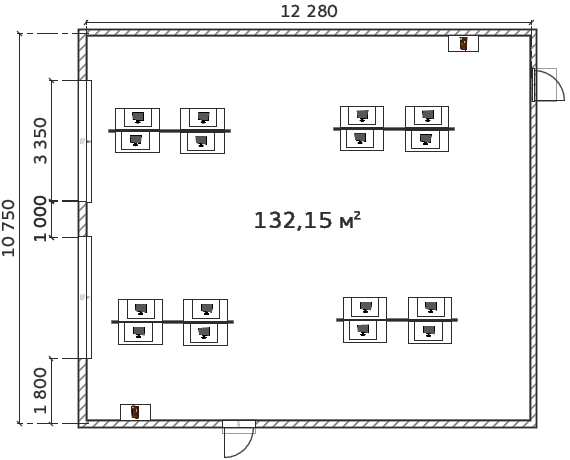
\includegraphics[scale=0.7]{labour/lab-plan.png}
            \end{center}
            \caption{Схема робочого приміщення}
            \label{fig:lab-plan}
    \end{figure}

    Геометричні параметри приміщення: ширина - 12.29 м, довжина - 10.75 м, висота - 3.5 м. Площа - 132.14 м кв., обєм - 462.49 м куб.
    У приміщенні передбачається розміщення 16 робочих місць обладнаних системними блоками та рідкокристалічними моніторами, живлення яких під'єднано до електричної мережі.

    Норматив ДНАОП 0.00-1.31-99\cite{lab-dnaop} передбачає на одного працюючого не менше 6 м кв. площі та не менше 20 м. куб. oб'єму.

    У офісному приміщенні, приведеному на рис.\ref{fig:lab-plan}, передбачено 16 робочих місць. Тоді відповідні параметри становлять 8.26 м. кв площі та при висоті стелі 3.5 м -  28.91 м куб. об'єму, що задовільняє норму.

    Для спрощення прокладки комунікацій стеля у приміщенні є підвісною. Для оздоблення стелі слід використовувати матеріали з коефіцієнтом відбиття 0.7 - 0.8, для стін 0.5 - 0.6.
    Покриття підлоги повинно бути матовим з коефіцієнтом відбиття 0.3 - 0.5. Поверхня підлоги повинна бути рівною і неслизькою.

    На робочому місці використовуються рідкокристалічні монітори (LCD) розміром 21 дюйм, які позбавлені багатьох недоліків (електромагнітне випромінювання, магнітне поле, мерехтіння і т.д.). На робочому місці присутній стіл глибиною 80 см, шириною 150 см та висотою 75 см від підлоги, присутній комп'ютерне крісло з можливістю налаштування висоти та регулювання кута наклону.

\subsection{Оцінка небезпечних і шкідливих виробничих факторів}
    \subsubsection{Мікрокліматичні умови}
    Категорія робіт, що виконуються на робочому місці є Іа - роботи, що виконуються сидячи і не потребують важкого фізичного навантаження ДСН 3.3.6.042-99\cite{lab-dsn42}. Роботи виконуються на постійному робочому місці.

    Мікроклімат у робочому приміщенні має відповідати наступним вимогам:
    \begin{itemize}
        \item оптимальна температура в холодний період року - 22..24 С, у теплий - 23..25 С;
        \item оптимальна відносна вологість 40-60\%;
        \item оптимальна швидкість руху повітря - 0.1 м/с;
        \item вміст шкідливих речовин у робочій зоні не повинен перевищувати ГДК.
    \end{itemize}

    Для підтримки оптимальної або допустимої температури в холодний період року приміщення повинно бути облаштоване системою водяного центрального опалення від місцевої або центральної теплової мережі, а в теплий період року - системою кондиціонування. Враховуючи, що у приміщенні встановлена підвісна стеля, може використовуватися спліт-система з внутрішнім блоком касетного типу.

    Вікна приміщення орієнтовані на північ, тому навіть у літній період не буде потрапляння прямих сонячних променів. Таке приміщення не потребує встановлення жалюзів на вікна.

    \subsubsection{Освітлення}

    На робочому місці проводяться зорові роботи із об'єктами 0.5 мм - 1 мм, контраст з об'єктів з фоном середній. Згідно з ДБН В.2.5-28-2006\cite{lab-dbn28} такий вид робіт відповідає розряду ІVг.

    Система освітлення у приміщенні суміщена, здійснюється як за допомогою природного світла з вікна, так і за рахунок штучних джерел на стелі. Сумарне освітлення робочої зони має бути таким, що сумарна освітленість на поверхні робочого столу становила 300 лк для розряду зорових робіт IVг (згідно ДБН В.2.5-28-2006\cite{lab-dbn28}).

    Природнє освітлення здійснюється за рахунок вікон орієнтованих на північ: два вікна, шириною 5 м та висотою 3 м. Загальна площа поверхні вікон 30 м кв.

    Штучне освітлення має здійснюватись переважно системою загального рівномірного освітлення. Рекомендованими є люмінесцентні лампи типу ЛБ - 32 лампи ЛБ-40 (цоколь G13) потужністю 40 Вт із застосуванням 8 світильників типу ЛВО 4х40 - світильник люмінісцентний, вбудований, для місць громадського користування на 4 лампи по 40 Вт кожна.
    Система загального освітлення повинна становити лінії світильників, розташованих збоку від робочих місць, паралельно лінії зору працюючих. План розміщення світильників штучного освітлення наведений на рис.\ref{fig:lab-plan-light}.

    \begin{figure}[h!]
            \begin{center}
                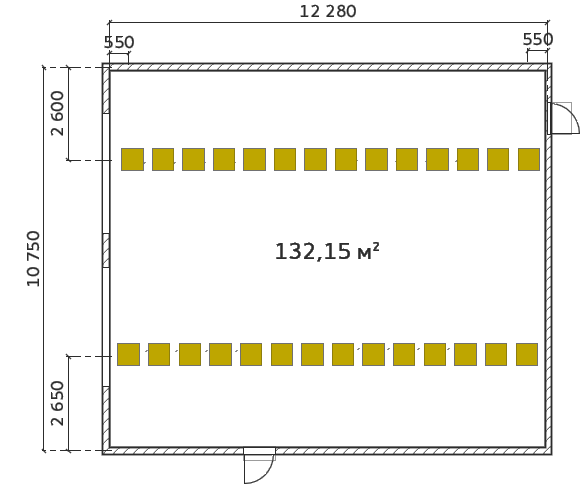
\includegraphics[scale=0.8]{labour/lab-plan-light.png}
            \end{center}
            \caption{Схема штучного освітлення робочого приміщення}
            \label{fig:lab-plan-light}
    \end{figure}

    Коефіцієнт природного освітлення (КПО) становить $e^{III}_n = 0.6$; відповідно
         до географічного розташування об'єкту у 4 поясі, коефіцієнт світлового клімату дорівнює $m = 0.9$, коефіцієнт сонячності клімату за умови що вікна орієнтовані на північ, а об'єкт росташований північніше 50 градусів, $C = 1.0$. Таким чином, нормативне значення природної освітленності
         становить:
         \[
             \textup{КПО} = e^{III} \cdot C \cdot m = 0.6 \cdot 0.9 \cdot 1.0 = 0,54
         \]

    Знайдемо площу вікон, що забеспечить нормоване значення КПО.

    \[
         S_B = \frac{S_{\textup{під}}}{100} \cdot \frac{e_n \cdot K_3 \cdot v_B \cdot K_{\textup{буд}}}{\tau \cdot r_1}
     \]

    Відношення довжини приміщення до його глибини $k_1 = \frac{10.75}{12.28} = 0,86$. Відношення глибини приміщення до висоти від рівня робочої поверхні до верхнього краю вікна $k_2 = \frac{12.28}{\frac{12.28}{3.5-0.75}} = 4,5$. Тоді світова характеристика вікон $v_B = 21$.

    $S_\textup{під} = 132,14 \textup{м}^2$ --- площа підлоги; $e_n = 0,81$ --- нормоване значення КПО; $ K_3 = 1,3$ --- коефіцієнт запасу; $ K_{\textup{буд}} = 1 $ --- коефіцієнт, що враховує
    затінення вікон будівлями, які розташовані навпроти; $\tau = 0,8 $ ---
    загальний коефіцієнт світопропускання; $r_1 = 1,2$ --- коефіцієнт, що
    враховує підвищення КПО при боковому освітленні завдяки світлу, яке
    відбивається від поверхонь приміщення (мінімальний). Підставляємо всі ці значення і
    отримуємо:
    \[
     S_B = \frac{132,14}{100} \cdot \frac{0,54 \cdot 1,3 \cdot 23 \cdot 1,0}{0,8 \cdot 1,2} = 29 \textup{м}^2
    \]

    Фактична площа більша ніж необхідна, тому природнє освітлення задовільняє норми.


        Розрахуємо відповідність штучного освітлення нормам. Для цього використаєм
        формулу світлового потоку:
        \[
            E_{\textup{ф}} = \frac{F_l \cdot N \cdot n \cdot \nu}{S_n \cdot K_3 \cdot Z}
        \],
        де  $F_{l}$ --- світловий потік однієї лампи в світильнику;
        $N$ --- кількість світильників; $n$ --- кількість ламп;
        $\nu$ --- коефіцієнт використання світлового потоку;
        $S_n$ --- площа приміщення; $K_3$ --- коефіцієнт запасу, розрахунковий
        коефіцієнт, що враховує зниження освітленності в процессі експлуатації
        внаслідок забруднення та старіння джерел світла, а також зниження
        показників відбиття поверхонь приміщення; $Z$ --- коефіцієнт нерівномірності
        освітлення.

        Показник приміщення за наступною формулою:
        \[
            i = \frac{ab}{h \cdot (a + b) = \frac{12,3 \cdot 10,75}{3,5 \cdot (12,3+10,75)}} = 1,63
        \]
        тоді коефіцієнт використання світового потоку становить $\nu = 58\% $.

        Світловий потік для використонуваних ламп становить 3200лм, а коефіціент
        нерівномірості 1.1

        Коефіцієнт запасу приймається рівним $K_3 = 1,3$.
        Підставляючи значення до основної формули методу світлового потоку отримаємо:
        \[
            E_{\textup{ф}} = \frac{3200 \cdot 8 \cdot 4 \cdot 0,58}{132,14 \cdot 1,3 \cdot 1.1} = 315 \textup{лм}
        \],
        що задовільняє норму в 300 лм.

    \subsubsection{Шум та вібрація}
    
        Згідно ДСН 3.3.6.037-99\cite{lab-dsn37} рівень шуму та рівні звукового тиску для програмістів та вчених (творчі професії), мають бути не більше 50 дБA. 

        Джерелами шуму є власний компютер та компьютери сусідів. Один комп'ютер з еквівалентим рівнем шуму одного - 40 дБА. Для пониження рівня шуму необхідно відрегулювати швидкість обертання кулерів центрального процесора та блоку живлення на допустимі значення. Це дозволяє знизити рівень шуму до 35 дБА.

        В одному блоку знаходиться 4 комп'ютера, сумарний шум $35 + 10lg(4) = 41$ дБА.
        В офісному приміщенні знаходяться 4 блоки, тому сумарний шум у приміщенні становить $$35 + 10lg(16) \approx 41 + 10lg(4) \approx 47 \textup{дБА}$$

        Отже, сумарний шум становить 47 дБА, що задовільняє норму 50 дБА.

        Вібрація на робочому місці не присутня.

    \subsubsection{Випромінювання}
    На робочому місці використовуються рідкокристалічні монітори (LCD), які позбавлені багатьох недоліків (електромагнітне випромінювання, магнітне поле, мерехтіння і т.д.).

    Рівні максимального електромагнітного випромінювання показані у таблиці \ref{tab:lab-waves}, причому максимальне значення
    електростатичного поля не повинно перевищувати 20 кВ/м.

    \begin{table}[h]
        \caption{Максимальні допустимі значення електромагнітного випромінювання на робочому місці}
        \begin{tabularx}{\textwidth}{| X | X | X |}
            \hline
            Частота електромагнітного поля (МГц) & Допустима напруженість (В/м) \\ \hline
            0.06 - 3     & 50                      \\ \hline
            3 - 30     & 20                      \\ \hline
            30 - 50    & 10                    \\ \hline
            50 - 300   & 5                      \\ \hline
        \end{tabularx}
        \label{tab:lab-waves}
    \end{table}

\subsection{Електрична безпека}
    У приміщенні характер виконуваних робіт пов'язаний з постійним використанням електроустановок(системних блоків, моніторів). Приміщення відноситься до класу без підвищеної небезпеки. Напруга у мережі становить 220В.

    Для забеспечення достатнього рівня електробезпеки, усі заземлені конструкції в приміщенні (батареї обігріву, водопровідні труби, кабелі з заземленим відкритим каналом), повинні бути захищені діелектричними щитками або сітками для недопущення потрапляння працівника під напругу. Для всієї проводки необхідно використовувати подвійну ізоляцію - основну та захисний короб.

    Необхідно забезпечити підключення заземлення всіх установок під напругою, обладнання в приміщенні повинно мати захист від короткого замикання та інших аварійних режимів, обладнання повинно підключатися виключно справними штепселями до стандартних електророзеток, лінія електромережі повинна бути окремою груповою трьохпроводною мережею, що складається з фазового, нульового робочого та нульового захисного провідників. Нульовий захисний провідник використовується для заземлення обладнання.

\subsection{Пожежна безпека}
    В приміщенні виконуються роботи із електричними установками, які можуть стати причиною пожежі. Забезпечення пожежної безпеки у приміщенні повинно здійснюватися комплексом заходів: організаційних, системи виявлення пожеж та системи пожежогасіння.
    До пожежонебезпечних матеріалів у розглянутому приміщенні можна віднести - тверді горючі речовини (дерев'яні меблі - столи, шафи), підісна стеля. Тоді згідно НАПБ Б.03.002-2007\cite{lab-napb} таке приміщення відноситься до категорії В(пожежонебезпечна).

    Потенційно можливі пожежі класу А -горіння твердих речовин, та класу Е - горіння електроустановок.

    Приміщення повинно відповідати вимогам системи попередження пожеж (максимальне використання негорючих матеріалів, застосування аварійного відключення на електроустановках, наявність систем виявлення пожежі, вогнегасників).

    Основні причини пожежі у приміщенні пов'язані з електричними приладами, напруга в яких не перевищує 380 В, необхідно встановити автоматичну дренчерну систему газового пожежогасіння з використанням хладона.

    Один димовий датчик контролює 30-50 м кв. Приміщення площею 132 м кв. має бути обладнане не менше ніж чотирма димовими датчиками сповіщення про пожежу.

\subsection{Техніка безпеки до виконання робіт}
    У приміщенні роботи проводяться з використанням пристроїв, що працюють під напругою: системні блоки, монітори. До виконання робіт допускаються виключно особи, що ознайомлені з усіма правилами безпеки.
    
    Виконання інструкцій техніки безпеки обов'язкове для всіх працівників.

    Перед початком робіт слід впевнитися, що у приміщенні немає проблем з електропроводкою. Заборонено починати роботи при наявності оголеної проводки.
    
    Заборонено включати електроприбори, якщо на робочому місці присутня волога(наприклад, розлита вода).
    
    Якщо під час включення комп'ютера виникли іскри або дим, слід негайно виключити електричний рубильник,
    при необхідності скористатися вогнегасником, та сповістити про це спеціальні служби.

    При потраплянні людини під напругу необхідно знеструмити відповідне робоче місце, надати першу долікарську допомогу і викликати «швидку».

    Не слід самостійно переключати будь-які запчастини, переєднувати проводи - це повинен робити фахівець.

    Не допускається наявність їжі та напоїв на робочому місці через загрози потрапляння води до електричних мереж.

% \section*{Висновки}
% \addcontentsline{toc}{section}{Висновки}
\newpage
\bigpart{Висновки}

\TBD
\renewcommand{\refname}{СПИСОК ВИКОРИСТАНИХ ДЖЕРЕЛ}
\bibliographystyle{ugost2008ls}
\bibliography{myrefs}

% \include{pz1/howto}
\end{document}
